\section{Restricciones}

Voy a dividir esta sección en varias subsecciones:

\subsection{Pistones}

Los pistones tienen las siguientes restricciones:

% fotos de las restricciones
\begin{figure}[H]
    \centering
    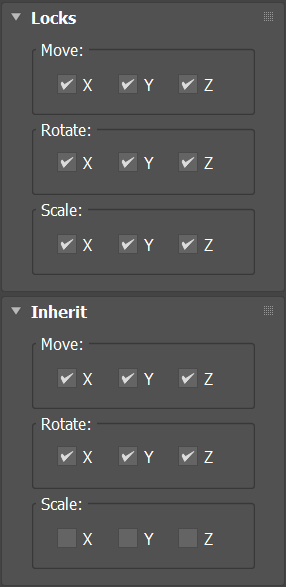
\includegraphics[width=0.2\textwidth]{imagenes/pistonlock.png}
    \caption{Restricciones aplicadas a los pistones.}
 \end{figure}

Como se puede ver, he bloqueado cualquier posibilidad de transformación, ya que el pistón es un objeto que debe seguir el movimiento de los demás. Además, he prohibido la herencia de escalado, ya que en el caso del pistón con la pala, se daba el caso de que se deformaba.

\bigskip

Asimismo, los cilindros que se estiran y comprimen (los que no hacen de soporte) tienen un \textit{LookAt Constraint} que se apuntan mutuamente para seguir el movimiento de manera realista.

\bigskip

Por último, los puntos de apoyo de los pistones tienen un \textit{Link Position} con la unión en el hueso que le corresponde.

\newpage

\subsection{Controladores}

Los controladores del brazo tienen las siguientes restricciones:

% foto de las restricciones
\begin{figure}[H]
    \centering
    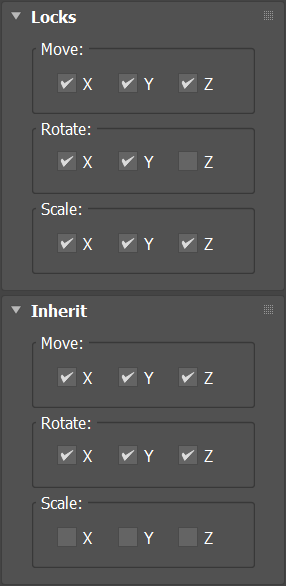
\includegraphics[width=0.2\textwidth]{imagenes/controladorverticallock.png}
    \caption{Restricciones aplicadas a los controladores.}
 \end{figure}

Así se prohíbe realizar movimientos del brazo no permitidos, como girar de izquierda a derecha. Además, las restricciones aplicadas al controlador que gira toda la excavadora prohíben giros incorrectos sobre cualquier otro eje que no sea el eje Z.

\subsection{Resto de figuras}

El resto de figuras tienen bloqueados todas las transformaciones, ya que son los controladores los que se encargan de mover los huesos de la grúa.